\begin{lstlisting}
Section 7.7: 5(a),6, 11
Section 7.8: 2,3
Section 7.9:8,9,11,13
\end{lstlisting}
\begin{exercise}
\begin{figure}[H]
\centering
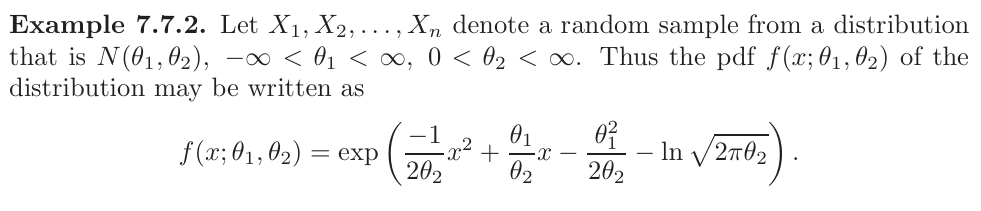
\includegraphics[width=\textwidth]{1-hw13-2025060122.png}
% \caption{}
\label{}
\end{figure}
\begin{figure}[H]
\centering
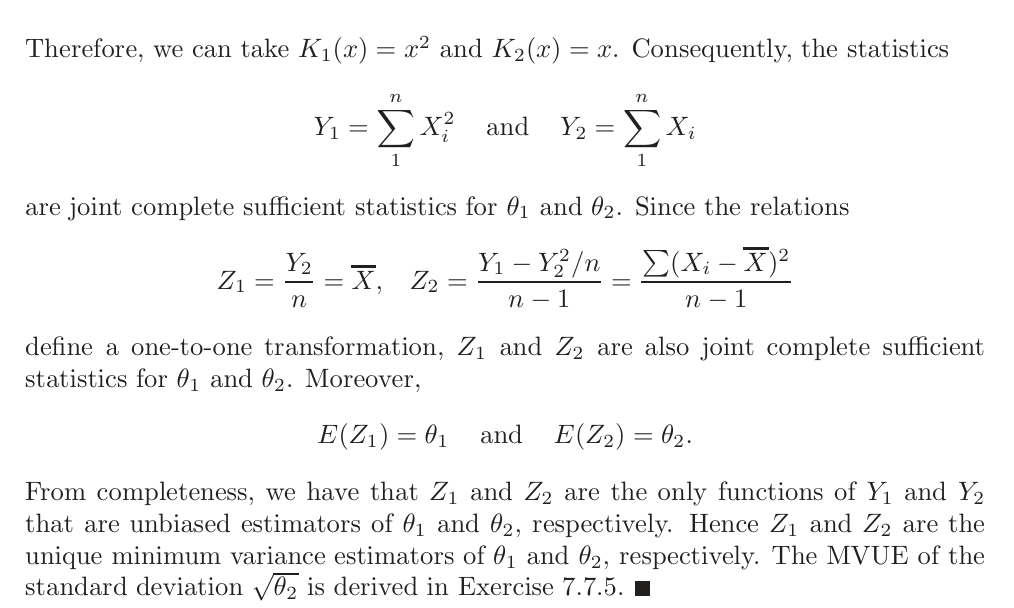
\includegraphics[width=\textwidth]{2-hw13-2025060122.png}
% \caption{}
\label{}
\end{figure}
\begin{figure}[H]
\centering
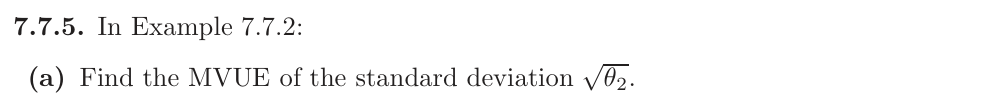
\includegraphics[width=\textwidth]{hw13-2025060122.png}
% \caption{}
\label{}
\end{figure}
\end{exercise}
\begin{figure}[H]
\centering
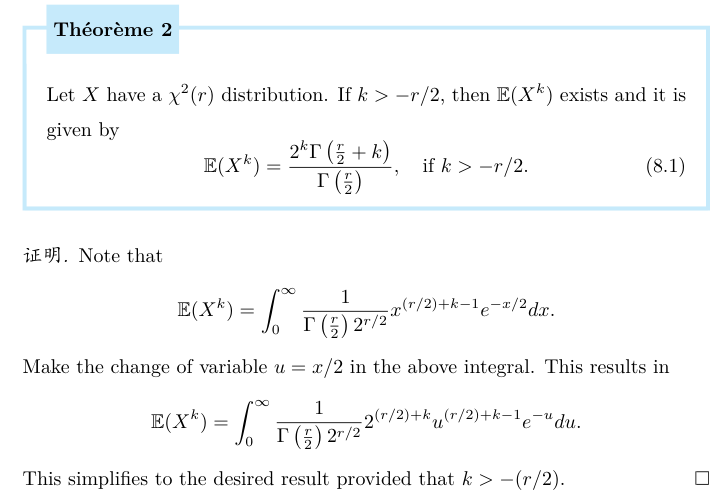
\includegraphics[width=\textwidth]{1-hw13-2025060200.png}
% \caption{}
\label{}
\end{figure}
\begin{figure}[H]
\centering
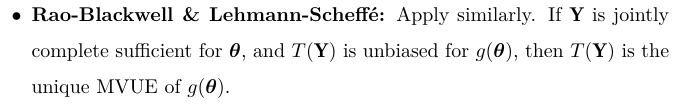
\includegraphics[width=\textwidth]{2-hw13-2025060200.png}
% \caption{}
\label{}
\end{figure}

Consider
\[
\mathbb{E}\underbrace{ \left[ \frac{\sqrt{ n-1 }\cdot\Gamma\left( \frac{n-1}{2} \right)}{\sqrt{ 2 }\cdot\Gamma\left( \frac{n}{2} \right)} \sqrt{ Z_2 }\right] }_{ \eqqcolon T(Y_1,Y_2) }=\sqrt{ \theta_2 }
\]
Thus the unique MVUE of $g(\theta_1,\theta_2)=\sqrt{ \theta_2 }$ is
\[
 \frac{\sqrt{ n-1 }\cdot\Gamma\left( \frac{n-1}{2} \right)}{\sqrt{ 2 }\cdot\Gamma\left( \frac{n}{2} \right)} \sqrt{ \frac{Y_1-Y_2^2/n }{n-1} }
\]
\begin{exercise}
\begin{figure}[H]
\centering
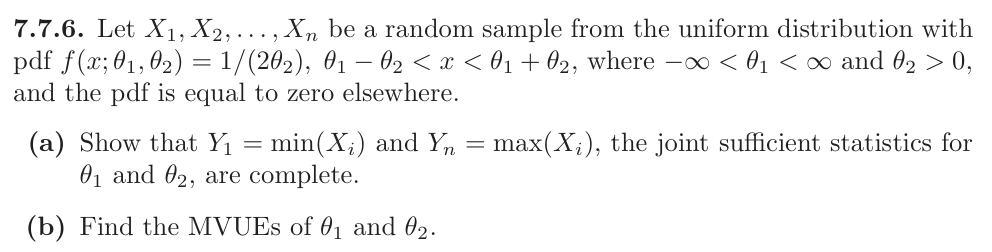
\includegraphics[width=\textwidth]{3-hw13-2025060122.png}
% \caption{}
\label{}
\end{figure}
\end{exercise}
\begin{figure}[H]
\centering
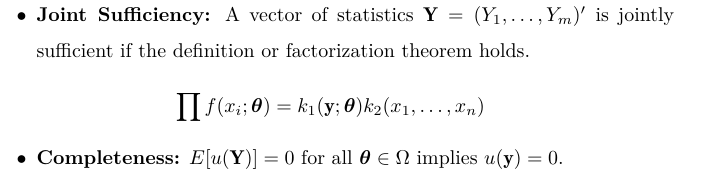
\includegraphics[width=\textwidth]{3-hw13-2025060200.png}
% \caption{}
\label{}
\end{figure}
(a)
\[
\prod f(x_i;\boldsymbol{\theta})=\prod\frac{1}{2\theta_2}\mathbb{1}_{\theta_1-\theta_2<x_i<\theta_1+\theta_2}=\frac{1}{2^{n}\theta_2^{n}}\mathbb{1}_{\theta_1-\theta_2<y_1\leq y_n<\theta_1+\theta_2}\eqqcolon k_1(\mathbf{y};\boldsymbol{\theta})\cdot \underbrace{ k_2(x_1,\dots, x_n) }_{ =1 }
\]
Thus $Y_1=\min(X_i)$ and $Y_n=\max(X_i)$ are joint sufficient statistics for $\theta_1,\theta_2$. Note that $Y_1,Y_2$ are dependent. In the support $\theta_1-\theta_2<y_1<y_n<\theta_1+\theta_2$,
\[
F(y_n)-F(y_1)=\frac{y_n-(\theta_1-\theta_2)}{2\theta_2}-\frac{y_1-(\theta_1-\theta_2)}{2\theta_2}=\frac{y_n-y_1}{2\theta_2}
\]
So
\[
f(\mathbf{y};\boldsymbol{\theta})=n(n-1)[F(y_n)-F(y_1)]^{n-2}f(y_1)f(y_n)=\frac{n(n-1)(y_n-y_1)^{n-2}}{(2\theta_2)^{n}}
\]
Suppose that $\mathbb{E}[u(\mathbf{Y})]=0$ for any $\boldsymbol{\theta}\in \Omega$, then
\[
\mathbb{E}[u(\mathbf{Y})]  =\int_{\theta_1-\theta_2}^{\theta_1+\theta_2 } \int_{y_1}^{\theta_1+\theta_2} u(y_1,y_n)\frac{n(n-1)(y_n-y_1)^{n-2}}{(2\theta_2)^{n}} \, \mathrm{d}y_n  \, \mathrm{d}y_1 
\]
Let $u=\theta_1-\theta_2,v=\theta_1+\theta_2$, then
\[
\int_{u}^{v} \int_{y_1}^{v}\underbrace{  u(y_1,y_n)(y_n-y_1)^{n-2} }_{ \eqqcolon K(y_1,y_n) } \, \mathrm{d}y_n  \, \mathrm{d}y_1=0 
\]
Then
\[
0=\frac{ \partial^2   }{ \partial u\partial v }\int_{u}^{v} \int_{y_1}^{v} K(y_1,y_n) \, \mathrm{d}y_n  \, \mathrm{d}y_1=K(u,v)\quad \text{a.e.}
\]
Since $y_n>y_1$, $(y_n-y_1)^{n-1}\neq0$ for $n\geq2$, thus $g(y_1,y_n)=0$ a.e. (this is the case when $n\geq2$. When $n=1$, $f(x_1;\theta_1,\theta_2)=\frac{1}{2\theta_2}\mathbb{1}_{\theta_1-\theta_2<x_1<\theta_1+\theta_2}$) We are done!

(b)
\[
f_{Y_1}(x)=\frac{n}{2^{n}\theta_2^{n}}(\theta_1+\theta_2-x)^{n-1}\mathbb{1}_{\theta_1-\theta_2<x<\theta_1+\theta_2}
\]
\[
f_{Y_2}(x)=\frac{n}{2^{n}\theta_2^{n}}(x-\theta_1+\theta_2)^{n-1}\mathbb{1}_{\theta_1-\theta_2<x<\theta_1+\theta_2}
\]
\[
\mathbb{E}(Y_1)=\frac{n}{2^{n}\theta_2^{n}}\int_{\theta_1-\theta_2}^{\theta_1+\theta_2} x(\theta_1+\theta_2-x)^{n-1} \, \mathrm{d}x =\frac{\theta _1 (n+1)-\theta _2 (n-1)}{n+1}
\]
\[
\mathbb{E}(Y_n)=\frac{n}{2^{n}\theta_2^{n}}\int_{\theta_1-\theta_2}^{\theta_1+\theta_2} x(x-\theta_1+\theta_2)^{n-1} \, \mathrm{d}x=\frac{\theta _1 (n+1)+\theta _2 (n-1)}{n+1} 
\]
Thus $\mathbb{E}\left( \frac{Y_1+Y_n}{2} \right)=\theta_1$, $\mathbb{E}\left[ \frac{n+1}{2n-2}(Y_n-Y_1) \right]=\theta_2$.
\begin{figure}[H]
\centering
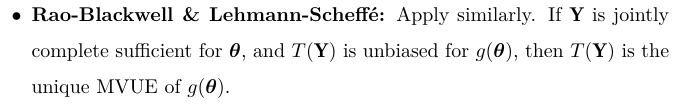
\includegraphics[width=\textwidth]{2-hw13-2025060200.png}
% \caption{}
\label{}
\end{figure}
Then $\frac{Y_1+Y_n}{2}$ is the unique MVUE of $\theta_1$, $\frac{n+1}{2n-2}(Y_n-Y_1)$ is the unique MVUE of $\theta_2$.

\begin{exercise}
\begin{figure}[H]
\centering
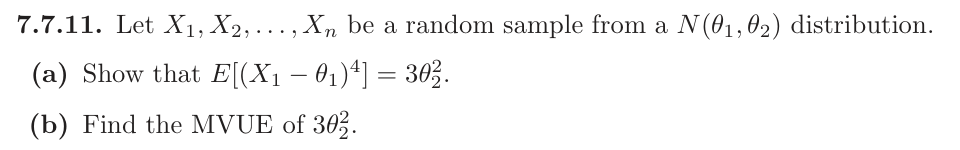
\includegraphics[width=\textwidth]{4-hw13-2025060122.png}
% \caption{}
\label{}
\end{figure}
\end{exercise}
(a)
\[
X_1\sim N(\theta_1,\theta_2)
\]
\[
f_{X_1}(x)=\frac{1}{\sqrt{ 2\pi\theta_2 }}\exp \left\{  -\frac{(x-\theta_1)^2}{2\theta_2}   \right\}
\]
\[
\begin{aligned}
\mathbb{E}[(X_1-\theta_1)^{4}] & =\int_{-\infty}^{\infty} (x-\theta_1)^{4}\cdot\frac{1}{\sqrt{ 2\pi\theta_2 }}\exp \left\{  -\frac{(x-\theta_1)^2}{2\theta_2}  \right\} \, \mathrm{d}x  \\
 & =\frac{4\theta_2^2}{\sqrt{ \pi }}\int_{-\infty}^{\infty} x^{4}e^{ -x^2 } \, \mathrm{d}x \\
 & = \frac{4\theta_2^2}{\sqrt{ \pi }}\cdot\frac{3}{4}\sqrt{ \pi } \\
 & =3\theta_2^2 
\end{aligned}
\]
Note that
\[
\int_{-\infty}^{\infty} x^{4}e^{ -x^2 } \, \mathrm{d}x =\left.\left[ \frac{ \partial^2   }{ \partial k ^2 }\left( \int_{-\infty}^{\infty} e^{ -kx^2 } \, \mathrm{d}x  \right) \right]\right|_{k=1}= \left.\left[ \frac{ \partial^2   }{ \partial k ^2 }\left(\sqrt{ \pi }\cdot k^{-\frac{1}{2}}\right) \right]\right|_{k=1}=\left.\left( \frac{3}{4}\sqrt{ \pi }k^{-\frac{5}{2}} \right)\right|_{k=1}=\frac{3}{4}\sqrt{ \pi }
\]
(b)
\begin{figure}[H]
\centering
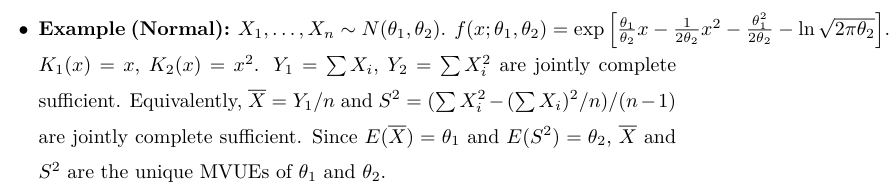
\includegraphics[width=\textwidth]{hw13-2025060216.png}
% \caption{}
\label{}
\end{figure}
\begin{figure}[H]
\centering
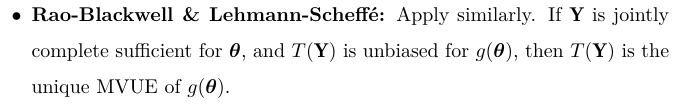
\includegraphics[width=\textwidth]{2-hw13-2025060200.png}
% \caption{}
\label{}
\end{figure}
$Y_1,Y_2$ are complete sufficient.

\begin{figure}[H]
\centering
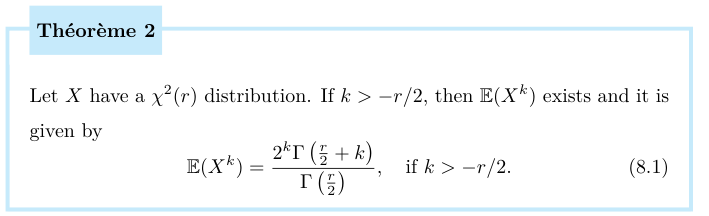
\includegraphics[width=\textwidth]{hw13-2025060217.png}
% \caption{}
\label{}
\end{figure}
By Student's theorem,
\[
(n-1)S^2/\theta_2\sim \chi^{2}(n-1)
\]
Then
\[
\mathbb{E}\left[ \frac{(n-1)^2(S^2)^2}{\theta_2^2} \right]=\frac{2^{2}\Gamma\left( \frac{n-1}{2}+2 \right)}{\Gamma\left( \frac{n-1}{2} \right)}=n^2-1
\]
Thus
\[
\mathbb{E}\left[ \frac{3n-3}{n+1}(S^2)^2 \right]=3\theta_2^2
\]
where
\[
S^2=\frac{1}{n-1}\left( Y_2-\frac{Y_1^2}{n} \right)
\]
Therefore the unique MVUE of $3\theta_2^2$ is
\[
\frac{3}{n^2-1}\left( Y_2-\frac{Y_1^2}{n} \right)^2
\]
\begin{exercise}
\begin{figure}[H]
\centering
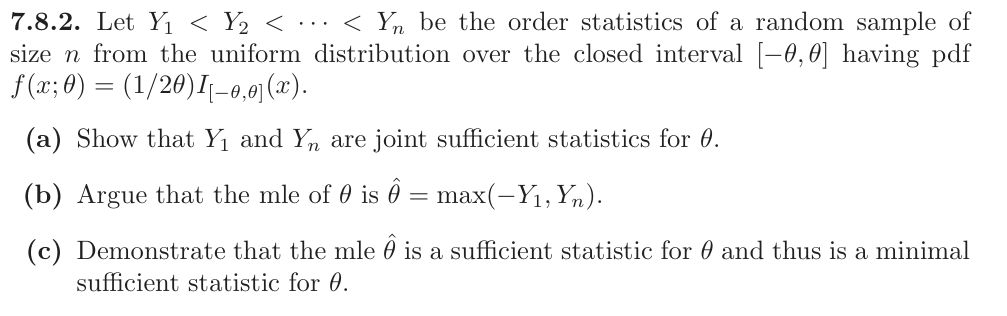
\includegraphics[width=\textwidth]{5-hw13-2025060122.png}
% \caption{}
\label{}
\end{figure}
\end{exercise}
(a)
\[
\prod f(x_i;\boldsymbol{\theta})=\prod\frac{1}{2\theta}\mathbb{1}_{-\theta\leq x_i\leq \theta}=\frac{1}{2^{n}\theta^{n}}\mathbb{1}_{-\theta\leq y_1\leq y_n\leq \theta}\eqqcolon k_1(\mathbf{y};\boldsymbol{\theta})\cdot \underbrace{ k_2(x_1,\dots, x_n) }_{ =1 }
\]
Thus $Y_1$ and $Y_n$ are joint sufficient statistics for $\theta$.

(b)
\[
L(\theta)=\prod_{i=1}^{n} \frac{1}{2\theta}\mathbb{1}_{-\theta\leq x_i\leq \theta}=\frac{1}{2^{n}\theta^{n}}\mathbb{1}_{-\theta\leq y_1\leq y_n\leq \theta}
\]
The smaller $\theta$ is, the larger $L(\theta)$ is. We have $\theta\geq-y_1$ and $\theta\geq y_n$, i.e. $\theta\geq \max(-y_1,y_n)$. Thus $\widehat{\theta}=\max(-Y_1,Y_n)$.

(c)
The likelihood function is
\[
L(\theta;\mathbf{x})=\frac{1}{2^{n}\theta^{n}}\mathbb{1}_{\theta\geq \max(-y_1,y_n)}
\]
Thus $\widehat{\theta}=\max(-Y_1,Y_n)$ is sufficient. We need to show $\widehat{\theta}$ is minimal.

Let $W_1<\dots<W_n$ be the order statistic for the random samples $Z_1,\dots, Z_n$. Then
\[
K(\mathbf{x},\mathbf{z};\theta)=\frac{L(\mathbf{x};\theta)}{L(\mathbf{z};\theta)}=\frac{\mathbb{I}(\theta\geq \max(-y_1,y_n))}{\mathbb{I}(\theta\geq \max(-w_1,w_n))}
\]
is independent of $\theta$ if and only if $\max(-y_1,y_n)=\max(-w_1,w_n)$. Thus $\widehat{\theta}$ is minimal.

\begin{exercise}
\begin{figure}[H]
\centering
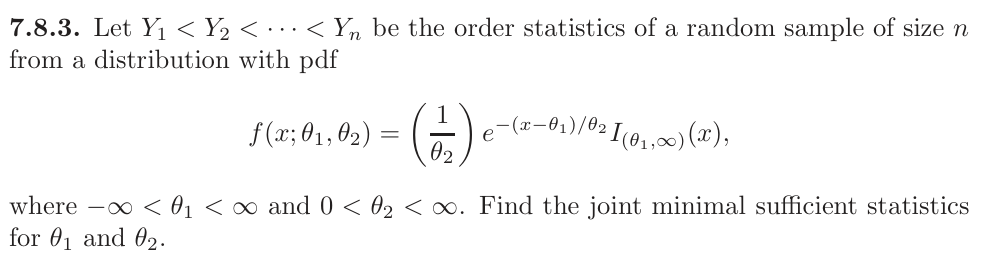
\includegraphics[width=\textwidth]{7-hw13-2025060122.png}
% \caption{}
\label{}
\end{figure}
\end{exercise}
\[
L(\mathbf{x};\boldsymbol{\theta})=\prod_{i=1}^{n} f(x_i;\boldsymbol{\theta})=\frac{1}{\theta_2^{n}}e^{ n\theta_1/\theta_2 }e^{ -\frac{1}{\theta_2} \sum x_i}\cdot \mathbb{I}(Y_1>\theta_1)
\]
Then $\sum X_i$ and $Y_1$ are sufficient.
\[
K(\mathbf{x},\mathbf{z};\boldsymbol{\theta})=\frac{L(\mathbf{x};\boldsymbol{\theta})}{L(\mathbf{z};\boldsymbol{\theta})}=\exp \left\{  -\frac{1}{\theta_2}\left( \sum x_i-\sum z_i \right)  \right\}\cdot\frac{\mathbb{I}(Y_1>\theta_1)}{\mathbb{I}(W_1>\theta_1)}
\]
is independent of $\boldsymbol{\theta}$ iff $\sum x_i=\sum z_i$ and $Y_1=W_1$. Therefore $\sum X_i$ and $Y_1$ are minimal sufficient.

\begin{exercise}
\begin{figure}[H]
\centering
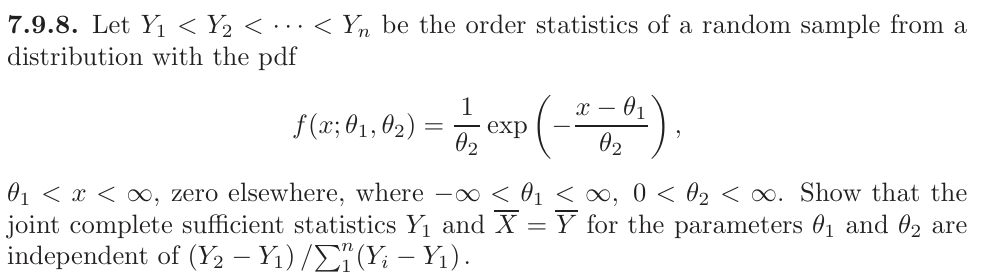
\includegraphics[width=\textwidth]{8-hw13-2025060122.png}
% \caption{}
\label{}
\end{figure}
\end{exercise}
Check:

\begin{enumerate}
	\item $Y_1$ and $\overline{X}$ are joint complete sufficient statistics.
	\item $Y_1$ and $\overline{X}$ are independent of $(Y_2-Y_1)/\sum_{i=1}^{n}(Y_i-Y_1)$.
\end{enumerate}

Since
\[
L(\mathbf{x};\boldsymbol{\theta})=\underbrace{ \theta_2^{-n}e^{ n\theta_1\theta_2 ^{-1} } }_{ =k_2(\boldsymbol{\theta}) }\cdot\underbrace{ \exp \left\{  -\theta_2^{-1}n\overline{X}  \right\}\cdot \mathbb{I}(Y_1>\theta_1) }_{ =k_1(\mathbf{y};\boldsymbol{\theta}) }
\]
$\overline{X}$, $Y_1$ are jointly sufficient. Next we show that they are complete.

Consider
\[
V\coloneqq \sum_{i=1}^{n} (X_i-Y_1)=n\overline{X}-nY_1
\]
There is a bijection between $(Y_1,\overline{X})$ and $(Y_1,V)$. Then it only suffices to show that $\mathbb{E}[u(Y_1,V)]=0$ implies $u\equiv0$ a.e.

\begin{itemize}
	\item Claim that $Y_1, V$ are independent. (这是 16 届 CMC 高年级组决赛概率论试题)
	\item $f_{Y_1}(y_1;\theta_1,\theta_2)=\frac{n}{\theta_2}\exp\left( -\frac{n(y_1-\theta_1)}{\theta_2} \right)\cdot \mathbb{I}(y_1>\theta_1)$.
	\item $f_{V}(v;\theta_2)=\frac{1}{\Gamma(n-1)\theta_2^{n-1}}v^{n-2}\exp\left( -\frac{v}{\theta_2} \right)\cdot \mathbb{I}(v>0)$ for $n\geq2$. (if $n=1$, $V=0$)
\end{itemize}

Suppose $\mathbb{E}[g(Y_1,V)]=0$ for all $\theta_1\in(-\infty,\infty )$ and $\theta_2>0$, then
\[
\int_{\theta_1}^\infty\int_0^\infty g(y_1,v)f_{Y_1}(y_1;\theta_1,\theta_2)f_V(v;\theta_2)dvdy_1=0
\]
\[
\int_{\theta_1}^\infty\frac{n}{\theta_2}e^{-n (y_1-\theta_1)/\theta_2}\left (\int_0^\infty g (y_1, v)\frac{v^{n-2}e^{-v/\theta_2}}{\Gamma (n-1)\theta_2^{n-1}}dv\right) dy_1=0
\]
Then
\begin{equation}
\int_{\theta_1}^{\infty} e^{ -ny_1/\theta_2 }K(y_1,\theta_2) \, \mathrm{d}y_1=0
\label{d3ba3f}
\end{equation}

where $K(y_1,\theta_2)\coloneqq \int_{0}^{\infty} g(y_1,v)v^{n-2}e^{ -v/\theta_2 } \, \mathrm{d}v$. Fix $\theta_2$, and differentiating \cref{d3ba3f} w.r.t. $\theta_1$, then
\[
e^{ -n\theta_1\theta_2 ^{-1} }K(\theta_1,\theta_2)=0\qquad \forall \theta_1\in(-\infty,\infty)
\]
By the property of Laplace Transform,
\[
g(y_1,v)v^{n-2}=0\qquad \text{a.e.}
\]
Thus $g(y_1,v)=0$ a.e. $Y_1,V$ are complete. Therefore $Y_1,\overline{X}$ are complete

We also need to show $Z\coloneqq\frac{Y_2-Y_1}{\sum_{i=1}^{n}(Y_i-Y_1)}$ is ancillary, thus by Basu theorem, $Y_1,\overline{X}$ are independent of $Z$.

We have known that $X_i=\theta_1+\theta_2W_i$ for random samples $W_i\sim \exp(1)$. The order statistics of $W_i$ is denoted by $W_{(i)}$. Then
\[
Z=\frac{(\theta_1+\theta_2W_{(2)})-(\theta_1+\theta_2W_{(1)})}{\sum_{i=1}^{n} (\theta_1+\theta_2 W_{(i)}-\theta_1-\theta_2 W_{(1)})}=\frac{W_{(2)}-W_{(1)}}{\sum_{i=1}^{n} (W_{(i)}-W_{(1)})}
\]
whose distribution does not depend on the parameter $\boldsymbol{\theta}$. We are done!

\begin{exercise}
\begin{figure}[H]
\centering
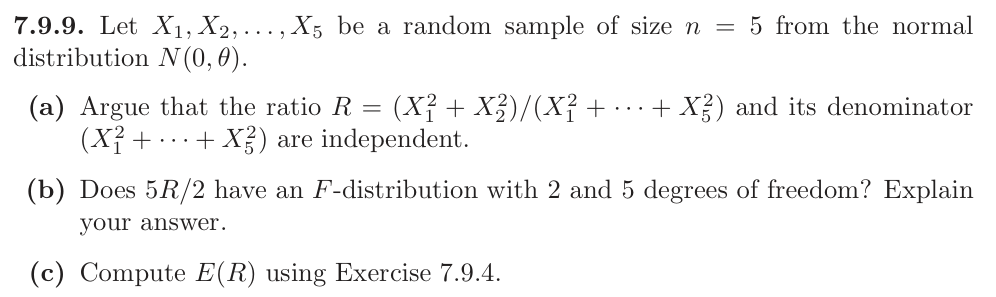
\includegraphics[width=\textwidth]{9-hw13-2025060122.png}
% \caption{}
\label{}
\end{figure}
\end{exercise}
(a) $Y_2=\sum X_i^2$ is complete sufficient. And
\[
R=\frac{\overbrace{ \left( \frac{X_1}{\theta} \right)^2+\left( \frac{X_2}{\theta} \right)^2 }^{ \sim \chi^{2}(2) }}{\underbrace{ \left( \frac{X_1}{\theta} \right)^2+\dots+\left( \frac{X_5}{\theta} \right)^2 }_{ \sim \chi^{2}(5) }}
\]
has distribution independent of the parameter $\theta$. By Basu theorem, $R$ and $(X_1^2+\dots+X_5^2)$ are independent.

(b)
No, because $\left( \frac{X_1}{\theta} \right)^2+\dots+\left( \frac{X_5}{\theta} \right)^2$ and $\left(\frac{X_1}{\theta} \right)^2+\left ( \frac{X_2}{\theta} \right)^2$ are not independent.

(c)
\begin{figure}[H]
\centering
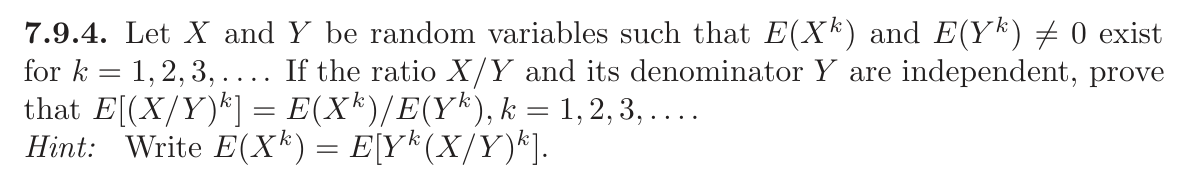
\includegraphics[width=\textwidth]{hw13-2025060300.png}
% \caption{}
\label{}
\end{figure}
\[
\mathbb{E}(R) =\frac{\mathbb{E}\left[ \left( \frac{X_1}{\theta} \right)^2+\left( \frac{X_2}{\theta} \right)^2 \right]}{\mathbb{E}\left[ \left( \frac{X_1}{\theta} \right)^2+\dots+\left( \frac{X_5}{\theta} \right)^2 \right]}  =\frac{2}{5}
\]
\begin{exercise}
\begin{figure}[H]
\centering
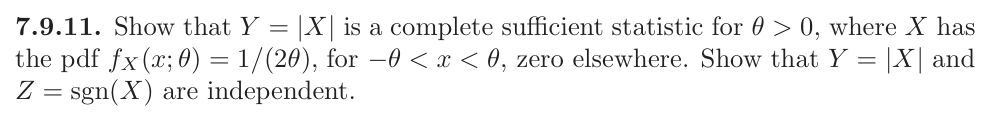
\includegraphics[width=\textwidth]{10-hw13-2025060122.png}
% \caption{}
\label{}
\end{figure}
\end{exercise}
$Z$ has pdf $p(-1)=\frac{1}{2}$, $p(1)=\frac{1}{2}$, thus is ancillary. It suffices to show that $Y$ is complete sufficient, by Basu theorem. We have
\[
f_{X}(x;\theta)=\frac{1}{2\theta}\cdot \mathbb{I}(\lvert X \rvert <\theta)
\]
thus $Y$ is sufficient. Suppose that $\mathbb{E}[u(Y)]=0$ for any $\theta>0$, then
\[
\int_{-\theta}^{\theta} \frac{1}{2\theta}\cdot u(\lvert x \rvert ) \, \mathrm{d}x =0
\]
i.e.
\[
\int_{0}^{\theta} u(\lvert x \rvert ) \, \mathrm{d}x=0
\]
Differentiate w.r.t. $\theta$, then we have $u(\lvert \theta \rvert)=0$ a.e. for any $\theta>0$. Thus $u\equiv0$ a.e. $Y$ is complete. Hence $Y$ and $Z$ are independent by Basu theorem.

\begin{exercise}
\begin{figure}[H]
\centering
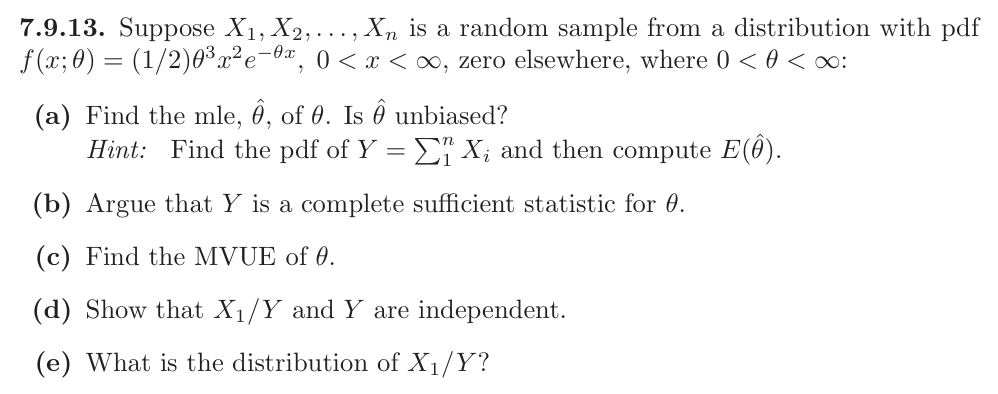
\includegraphics[width=\textwidth]{11-hw13-2025060122.png}
% \caption{}
\label{}
\end{figure}
\end{exercise}
(a)
\[
\ell(x;\theta)=2\sum_{i=1}^{n} \log x_i-\theta \sum_{i=1}^{n} x_i+3n\log\theta-n\log2
\]
\[
\frac{ \partial \ell(x;\theta) }{ \partial \theta }=-\sum_{i=1}^{n} x_i+3n\cdot\frac{1}{\theta}=0
\]
Then $\widehat{\theta}=\frac{3n}{Y}$, where $Y=\sum_{i=1}^{n}X_i$. $X_i\sim\Gamma(3,\theta ^{-1})$. Then $Y\sim\Gamma(3n,\theta ^{-1})$.
\[
\mathbb{E}(\widehat{\theta})=\mathbb{E}\left( \frac{3n}{Y} \right)=\int_{0}^{\infty} \frac{3n}{y}\cdot\frac{1}{\Gamma(3n)}\theta^{3n}y^{3n-1}e^{ -\theta y } \, \mathrm{d}y=\frac{3n\theta}{3n-1}
\]
Thus $\widehat{\theta}$ is not unbiased.

(b)
\[
f(x;\theta)=\exp(-\theta x+2\log x+3\log\theta-\log2)
\]
is regular exponential class, where $K(x)=x$. Then the statistic $Y=\sum_{i=1}^{n}K(X_i)=\sum_{i=1}^{n}X_i$ is a complete sufficient statistic for $\theta$.

(c)
\begin{figure}[H]
\centering
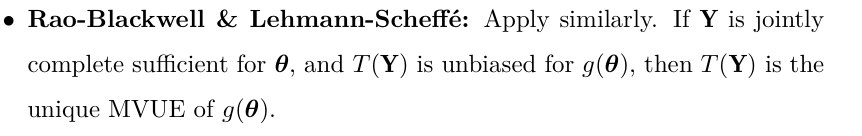
\includegraphics[width=\textwidth]{hw13-2025060301.png}
% \caption{}
\label{}
\end{figure}
The MVUE is
\[
\frac{3n-1}{Y}
\]
(d)
$X_i=\theta Z_i$ where $Z_i\sim\Gamma(3,1)$. Then $Y=\theta \sum_{i=1}^{n}Z_i$. Thus
\[
\frac{X_1}{Y}=\frac{Z_1}{\sum_{i=1}^{n} Z_i}
\]
has distribution not depending on $\theta$. By Basu theorem, since $Y$ is complete sufficient, $X_1/Y$ and $Y$ are independent.

(e)
\begin{figure}[H]
\centering
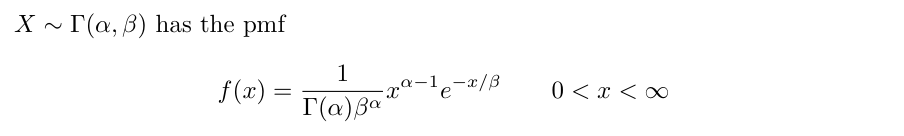
\includegraphics[width=\textwidth]{hw13-2025060310.png}
% \caption{}
\label{}
\end{figure}
Let $W\coloneqq Z_2+\dots+Z_n\sim\Gamma(3n-3,1)$, $(u,v)=\left( \frac{z}{z+w},z \right)$, $(U,V)=\left( \frac{Z_1}{Z_1+W},Z_1 \right)$. Then
\[
\begin{aligned}
f_{U,V}(u,v) & =f_{Z_1,W}\left( v,\frac{v}{u}-v \right)\left\lvert  \frac{ \partial \left( v,\frac{v}{u}-v \right) }{ \partial (u,v) }   \right\rvert  \\
 & =\frac{v^{3n-1}}{2u^2}\cdot\frac{1}{(3n-4)!}\left( \frac{1}{u}-1 \right)^{3n-4}e^{ -\frac{v}{u} }
\end{aligned}
\]
Then the distribution of $X_1/Y$ is
\[
\begin{aligned}
f_{U}(u) & =\int_{0}^{\infty} f_{U,V}(u,v) \, \mathrm{d}v \\
 & =\int_{0}^{\infty} \frac{v^{3n-1}}{2u^2}\cdot\frac{1}{(3n-4)!}\left( \frac{1}{u}-1 \right)^{3n-4}e^{ -\frac{v}{u} } \, \mathrm{d}v   \\
 & =\frac{(1-u)^{3n-4}u^2(3n)!}{2(3n-4)!}
\end{aligned}
\]
where $u\in(0,1)$.
